%!TeX root= ../thesis.tex
\setcounter{section}{0}
\section{Introduction}
	La prise de décision collective est un processus dans lequel les préférences individuelles sont agrégées pour former un choix collectif unique. Cette définition large permet à de nombreux cas, qui semblent très différents les uns des autres, d'entrer dans cette catégorie.
	Parmi les exemples, citons les \textit{problèmes d'allocation équitable}\textemdash qui traite du problème de la répartition équitable de certaines ressources entre des individus qui ont des intérêts différents, par exemple l'allocation de maisons, la création d'un horaire de travail, etc.\textemdash \textit{problèmes d'appariement}\textemdash qui traite du problème de l'appariement d'individus de deux groupes distincts en tenant compte de leurs préférences, par exemple, des étudiants aux écoles, des locataires aux maisons etc.\textemdash 
	et \textit{problèmes d'agrégation de jugements}\textemdash qui tentent de regrouper les croyances de différents individus en un jugement qui reflète la société en tant qu'entité unique.
	Dans cette thèse, nous nous concentrerons sur un autre exemple de prise de décision collective : le \textit{vote}. Étant donné un ensemble d'individus qui expriment leurs préférences sur un ensemble donné de candidats, comment choisir le \textit{meilleur} candidat pour le groupe ? Il s'agit d'un dilemme très ancien qui a été affronté de multiples fois au cours des siècles et que nous allons aborder tout au long de ce manuscrit.
	Comme nous allons le voir, la réponse dépend de nombreux facteurs, tels que les informations dont nous disposons\textemdash connaissons-nous les préférences de tous les électeurs par rapport à tous les candidats ?\textemdash et les propriétés que nous voulons que le résultat satisfasse\textemdash qu'entendons-nous par le meilleur candidat ? Qui décide de ce qui est le meilleur ?
	
	Une méthodologie importante dans notre travail consiste à définir les propriétés souhaitables que nous voulons qu'une règle satisfasse. Cela nous permet, d'une part, de diviser les règles d'agrégation en classes de méthodes satisfaisant les mêmes propriétés, et, d'autre part, de faire le processus inverse : partir d'une méthode déjà définie pour aider le décideur à comprendre ses propriétés.
	Le manque d'information et l'aide aux décideurs sont deux des thèmes explorés au cours de ce travail.
	
	Nous avons mentionné l'analyse des processus d'agrégation par la définition de desiderata, mais cette approche axiomatique est très récente et n'a commencé qu'après la publication de la thèse de doctorat de Kenneth \citet{Arrow1951}.
	La théorie des processus de prise de décision collective est cependant beaucoup plus ancienne et, comme l'a écrit \citet{McLean1990}, \say{la théorie du vote est connue pour avoir été découverte trois fois et perdue deux fois}. En partant des premières traces des processus de décision, nous décrivons le début et l'évolution de la théorie du choix social. 
	
	\paragraph{Questions de recherche et contributions.}
	En étudiant l'histoire des méthodes d'agrégation, nous avons réalisé qu'à partir d'un large éventail de procédures, nous pouvons identifier des classes dont les éléments satisfont des propriétés communes. Étant donné une méthode, nous pouvons analyser les axiomes qu'elle satisfait.
	L'intérêt de cette démarche est que nous pouvons aussi faire l'inverse : étant donné certaines préférences sur les propriétés que la règle doit respecter, nous pouvons aider le décideur à définir la méthode d'agrégation qu'il souhaite. 
	C'est précisément l'un des points sur lesquels nous allons nous concentrer : 
	\begin{itemize}
		\item comment pouvons-nous aider le décideur à définir formellement une règle électorale sur la base de préférences génériques sur ses propriétés ?
	\end{itemize}
	Dans \Cref{ch:minimax}, nous étudions une situation dans laquelle un comité de non-experts doit décider comment agréger les préférences des électeurs. 
	Supposons que le comité attribue un score à chaque position dans l'ordre des préférences des électeurs. Ainsi, par exemple, le premier classé obtient 10 points, le second 5, etc.
	Imaginez maintenant que le comité souhaite que le score du meilleur choix soit \say{beaucoup plus élevé} que celui du troisième meilleur choix.
	Comment traduire ce "beaucoup plus" en une règle de vote ? Qu'est-ce que cela signifie exactement ?
	Dans cette thèse, nous nous concentrons sur une classe particulière de règles, les \textit{Règles de notation positionnelle} \textemdash que nous décrivons en détail dans \Cref{ch:preliminaries} \textemdash et développons une méthode pour poser des questions au comité en termes de choix des gagnants dans un exemple de profil. 
	Ainsi, nous transformons une question complexe impliquant des différences de poids entre des positions consécutives en des questions auxquelles un comité humain peut plus facilement répondre, telles que "qui devrait gagner dans ce profil" ? De la réponse à cette question, nous déduisons la réponse à la question initiale.
	
	Un autre problème important lors du choix d'une règle de vote est son coût. C'est un point que nous retrouvons également dans notre première question de recherche. 
	Dans ce cas, il est représenté par le coût cognitif pour les non-experts de formaliser une règle de vote sur la base de certaines préférences génériques. Mais, comme nous le savons, le coût est également lié aux électeurs lorsqu'ils doivent ordonner un grand ensemble de préférences, et au calcul de la transmission de toutes ces informations.
	Cette prise de conscience nous amène à étudier les stratégies d'élicitation des préférences des électeurs :
	\begin{itemize}
		\item comment pouvons-nous acquérir les informations les plus pertinentes au moindre coût ?
	\end{itemize}
	Nous étudions cette question pour différentes règles de vote (règles de notation positionnelle et jugement majoritaire) dans \Cref{ch:minimax,ch:MJ}. En particulier, dans \Cref{ch:minimax}, nous combinons cette question de recherche avec la première et nous essayons de comprendre si, dans un contexte d'information nulle, l'imbrication de l'élicitation des préférences des électeurs et de l'élicitation de la règle de vote donne de meilleurs résultats qu'une approche plus linéaire. 
	Dans \Cref{ch:MJ}, nous étudions des scénarios concrets tirés de situations de vote réelles, dans lesquels les préférences des électeurs sont obtenues en posant un nombre donné de questions aléatoires aux électeurs. Entre autres, nous cherchons comment identifier le nombre minimum de questions à poser pour que la probabilité d'obtenir le gagnant, en utilisant la règle du jugement majoritaire, soit élevée.
	
	Nous avons commencé à nous demander comment différentes situations pouvaient justifier l'utilisation de différentes règles de vote qui cherchent à atteindre le même objectif.
	Dans la littérature, diverses notions de compromis ont été proposées, et avec elles diverses règles de vote qui tentent plus ou moins de mettre en œuvre ces définitions.
	Lorsque nous parlons de compromis, ce que nous entendons dépend beaucoup du contexte. Lorsque nous voulons décider où dîner, nous sommes probablement d'accord pour que les électeurs essaient de trouver un terrain d'entente, même si le résultat ne s'avère pas être un compromis. C'est le cas avec certaines règles de vote dont nous parlerons plus tard, comme le Fallback Bargaining, où il peut arriver que le résultat soit le meilleur choix pour certains électeurs, mais qu'il déplaise à beaucoup d'autres.
	Cependant, lorsque nous avons affaire à des contextes où l'égalitarisme \textemdash que nous interpréterons comme le fait que tout le monde concède également \textemdash est une préoccupation majeure, cette notion de compromis n'est plus acceptable.
	Sur ces bases, nous développons les fondements de notre concept de compromis :
	\begin{itemize}
		\item comment pouvons-nous définir la notion de compromis où chaque électeur concède de manière aussi égale que possible ?
	\end{itemize}
	Dans \Cref{ch:compromise}, nous abordons cette question et analysons quelles règles existantes, le cas échéant, répondent à cette nouvelle définition. Nous verrons que différentes définitions ont un sens dans différents contextes et que l'une n'est pas nécessairement meilleure que l'autre.
	
	\paragraph{Organisation de la thèse}
	\Cref{ch:preliminaries} rassemble les notions importantes qui sont à la base des thèmes abordés dans cette thèse et qui reviendront de manière récurrente dans les chapitres suivants. Nous y décrivons la différence entre le vote avec différents types de scrutins : les scrutins classés, que nous utiliserons dans \Cref{ch:minimax,ch:compromise}, et les scrutins notés, que nous considérerons dans \Cref{ch:MJ}. Nous allons décrire les règles de vote que nous utiliserons dans nos contributions et certains des axiomes qui les caractérisent.
	
	Dans \Cref{ch:literature}, en utilisant la même approche que dans cette introduction, nous fouillerons dans le passé pour positionner notre travail. En particulier, dans \Cref{sec:litCMP}, en partant de la signification du compromis, nous retraçons son utilisation à travers l'histoire. Nous analysons les définitions qui ont été données des règles de compromis dans la théorie du choix social et soulignons comment certaines d'entre elles ne représentent pas certaines idées du compromis. Nous montrons comment notre approche s'inscrit dans cette littérature. 
	Constatant que la règle du jugement majoritaire est considérée comme une forme de compromis dans la littérature, nous approfondirons cette règle dans \Cref{sec:litMJ}. Nous étudierons son introduction, ses utilisations et aussi ses critiques.
	Comme dernier sujet de ce chapitre, nous couvrons dans \Cref{sec:litMNMX} un autre aspect important de cette thèse : l'élicitation des préférences. En effet, si jusqu'à présent on a supposé connaître les préférences des électeurs et la procédure de vote, cela ne peut être considéré comme acquis. L'élicitation des préférences est un problème bien étudié et nous décrirons les différentes approches par lesquelles il a été abordé dans la littérature. En outre, nous décrirons comment il a été abordé dans différents domaines, notamment dans la littérature sur l'aide à la décision et l'apprentissage automatique, et les similitudes avec notre approche.
	
	\Cref{part:contributions} inclut nos contributions. Plus précisément, \Cref{ch:minimax} est un article publié dans une conférence internationale \citep{Napolitano2021} et \Cref{ch:compromise} est un article publié dans une revue \citep{Cailloux2022}. \Cref{ch:uml} accompagne \Cref{ch:minimax} en décrivant le code fourni à l'appui de la contribution. 
	Enfin, \Cref{ch:MJ} est une contribution originale, non encore publiée, dont le but est d'étudier les conséquences du processus d'élicitation dans une situation de vote utilisant le jugement majoritaire.
	
	Pour conclure, \Cref{ch:conclusion} fournit un résumé des contributions de cette thèse et quelques perspectives pour les directions futures.


\section*{Contributions}

\section{Simultaneous Elicitation of PSR and Agent Preferences}
	Le cadre classique du choix social suppose une information complète sur les ordres de préférence de tous les électeurs, et sur le mécanisme de vote lui-même. Mais dans quelle mesure cette hypothèse est-elle raisonnable ?
	Si l'ensemble des alternatives est très vaste, il n'est pas raisonnable d'attendre des électeurs qu'ils fournissent un ordre complet de leurs préférences. D'abord d'un point de vue cognitif : des études de psychologie expérimentale décrivent comment, dans de nombreuses situations, nos préférences ne sont pas prédéfinies, mais que nous les construisons seulement au moment où nous devons les exprimer \citep{Lichtenstein2006}. Demander aux électeurs d'exprimer leurs préférences lorsque l'éventail de choix est très large peut entraîner divers problèmes, tels que la confusion et une faible participation.
	Deuxièmement, mais non moins important, cela représente un énorme coût de communication. \citet{Conitzer2005} ont étudié la complexité de communication de certaines des règles de vote les plus courantes et, pour chacune d'entre elles, ont fourni une limite supérieure et inférieure sur le nombre de bits d'information que les électeurs doivent communiquer avant que la règle puisse sélectionner un gagnant. D'autres mesures existent, comme le nombre de questions auxquelles les électeurs doivent répondre avant que la règle puisse déterminer un gagnant. Cette approche a été utilisée par \citet{Procaccia2008} pour déterminer le nombre minimum de questions permettant de sélectionner le gagnant de Condorcet.
	Dans les élections présidentielles, par exemple, nous avons tendance à préférer la précision au coût, mais ce n'est pas vrai dans toutes les applications. Lorsqu'il s'agit de choisir un restaurant pour dîner avec des amis, nous nous contenterons probablement d'un gagnant approximatif plutôt que de devoir passer toute la soirée à classer tous les restaurants de la ville.
	
	Cette observation a motivé plusieurs travaux supposant des ordres de préférence partiels : 
	un des premiers travaux est celui de \citet{Conitzer2005} qui a étudié la complexité de la communication lors de l'utilisation de différentes règles de vote ;
	\citet{Konczak05} a étudié le calcul des gagnants possibles et nécessaires pour différentes règles de vote ;
	\citet{Xia2008} ont ensuite montré que, si l'identification d'un co-gagnant nécessaire dans les règles de notation est polynomiale, la détermination des co-gagnants possibles est NP-dure ;
	D'autres résultats de complexité ont été donnés par \citet{Walsh2007} et \citet{Pini2007}.
	
	Puisque dans de nombreuses situations pratiques, il y aurait trop de gagnants possibles mais pas de gagnants nécessaires, plusieurs travaux ont abordé le problème de l'élicitation des préférences des agents en utilisant une variété d'approches (regret minimax, méthodes bayésiennes, etc.) dans le but de converger vers un gagnant nécessaire : \citep{Naamani-Dery2015,Kalech2011,Lu2011,Pini2009,Benabbou2016,Dey2016_2}. Parmi ceux-ci, \citet{Walsh2009} et \citet{Conitzer2009} ont analysé quand arrêter le processus d'élicitation.

	Une deuxième préoccupation concerne la capacité de la personne ou l'organisation qui supervise le processus de vote à fournir une définition précise de la règle de vote, ce qui suggère l'assouplissement de la deuxième hypothèse. En effet, il est souvent difficile pour des non-experts de formaliser une règle de vote sur la base de quelques préférences génériques sur une méthode d'agrégation souhaitée. 
	Nous donnons ici deux exemples de telles situations.
	
	Considérons, comme premier exemple, une commission qui est sur le point d'embaucher un nouvel employé dont les performances sont évaluées par plusieurs experts. Les membres de la commission peuvent ne pas avoir de règle de vote en tête au début du processus et ne pas vouloir se mettre d'accord sur une règle de vote spécifique. Cependant, ils pourraient être disposés à répondre à quelques questions exigeant de sélectionner le gagnant parmi des profils spécifiques. 
	
	Considérons, comme deuxième exemple, le processus d'évaluation d'une conférence où le meilleur article doit être élu. Les agents expriment leurs préférences sur les articles qu'ils ont évalués, mais ils ne sont pas conscients de la règle de vote que le président du programme appliquera lorsqu'il les regroupera. Néanmoins, les évaluateurs sont toujours prêts à participer au processus. De plus, le CP peut ne pas avoir de règle de vote spécifique en tête, et il lui sera difficile de fournir un vecteur de notation précis si on le lui demande. Peut-être croit-elle fermement que le fait d'être classé une fois en première position a "beaucoup plus" de valeur que le fait d'être classé deux fois en deuxième position, mais ne sait pas exactement de combien (bien qu'elle puisse juger des cas d'exemple).
	
	Nous nous concentrons sur les règles de notation positionnelle avec des poids convexes, qui sont une méthode particulièrement courante utilisée pour agréger les classements. 
	Nous développons des méthodes, basées sur la notion de regret minimax, pour déterminer un "gagnant" robuste en cas d'incertitude à la fois sur la règle de vote et sur les préférences des agents.
	Nous fournissons des méthodes d'élicitation incrémentales qui, à chaque étape de l'élicitation, interrogent l'un des agents ou le président, et nous discutons de plusieurs heuristiques pour choisir des questions qui réduisent rapidement le regret.
	Les réponses aux questions sont encodées sous forme de contraintes ; les questions aux agents sont des comparaisons entre des paires d'alternatives tandis que les questions au président demandent de sélectionner un gagnant parmi un profil synthétique.

	\paragraph{Conclusions.}
	Notre approche est évaluée sur des simulations avec des ensembles de données synthétiques et réelles où la règle de vote et les préférences de l'agent sont initialement inconnues du système et progressivement révélées par des questions. Nous supposons que le président est humain, donc capable de répondre à des questions sur un nombre limité d'alternatives, et nous nous concentrons donc sur des situations de choix social à petite échelle. Nous comparons l'efficacité de plusieurs stratégies de questionnement basées sur la connaissance actuelle de la règle et des préférences. Pour résumer nos contributions : 
	
	1) Nous fournissons un nouveau mécanisme pour éliciter une règle de vote en traduisant des questions abstraites sur les poids en un choix d'une alternative étant donné un profil concret. 
	Supposons, par example, que nous voulions poser la question suivante à la commission : $w_{2} - w_{3} ≥ 2 (w_{3} - w_{4})$. Cela signifie que nous voulons savoir si la différence de poids entre la deuxième et la troisième position est supérieure ou égale au double de la différence entre la troisième et la quatrième position. Nous montrons le profil de la figure \ref{fig:profileQstCommFrench} à la commission et demandons qui devrait gagner (chaque colonne est la préférence d'un agent).
	Les deux $a$ et $b$ ont des scores supérieurs à $c$ et $d$ pour tous les poids convexes, donc soit $a$ soit $b$ seront choisis selon notre hypothèse ; et $s(a) ≥ s(b) ⇔ w_2 + 2 w_4 ≥ 3 w_3$.
	La figure \ref{fig:profileQstCommCompactFrench} représente le même profil en utilisant une vue compressée, les chiffres en gras indiquant le nombre d'agents ayant la préférence dans la colonne correspondante.
	
	\begin{figure}
		\centering
		\caption{Profil représentant une question posée à la commission sous forme étendue (a) et compacte (b).}
		\begin{subfigure}[b]{0.49\textwidth}
			\begin{center}
				$
				\begin{array}{ccccccccc}
					c&d&d&a&a&a&b&b&b\\
					a&c&c&b&b&b&a&a&a\\
					b&b&b&c&c&c&d&d&d\\
					d&a&a&d&d&d&c&c&c\\
				\end{array}
				$
			\end{center}
			\caption{}
			\label{fig:profileQstCommFrench}
		\end{subfigure}
		\hfill
		\begin{subfigure}[b]{0.49\textwidth}
			\begin{center}
				$
				\begin{array}{cccc}
					\mathbf{1}&\mathbf{2}&\mathbf{3}&\mathbf{3} \\
					c&d&a&b\\
					a&c&b&a\\
					b&b&c&d\\
					d&a&d&c\\
				\end{array}
				$
			\end{center}
			\caption{}
			\label{fig:profileQstCommCompactFrench}
		\end{subfigure}
	\end{figure} 
	
	
	2) Nous montrons qu'avec notre méthode d'élicitation, il est possible d'atteindre un faible regret avec un nombre raisonnable de questions, voir \Cref{fig:linearityFrench}
	
	\begin{figure}
		\caption{MMR moyen (normalisé par $n$) après $k$ questions avec la stratégie pessimiste pour différents ensembles de données.}
		\label{fig:linearityFrench}
		\centering
		\begin{tikzpicture}[scale=1.2]
			\pgfplotsset{
				every axis legend/.append style={
					at={(0.5,1.1)},
					anchor=south
				},
			}
			\begin{axis}[
				y=80,
				legend columns=3,
				xlabel=Number of Questions,
				ylabel=MMR/n,
				ytick={0,0.5,1},
				xtick distance=100,
				xtick pos=left,
				ymajorgrids=true,
				ytick style={draw=none},
				ymin=0,
				ymax=1,
				xmin=0,
				xmax=1000,
				yticklabels={0,0.5,1},
				legend style={font=\footnotesize}]
				
				\addlegendimage{mark=halfsquare right*,brown,mark size=2}
				\addlegendimage{mark=diamond*,red,mark size=2}
				\addlegendimage{mark=pentagon*,cyan,mark size=2}
				\addlegendimage{mark=halfcircle*,violet,mark size=2}
				\addlegendimage{mark=*,pink,mark size=2}
				\addlegendimage{mark=triangle*,green,mark size=2}
				\addlegendimage{mark=halfsquare left*,blue,mark size=2}
				\addlegendimage{mark=square*,teal,mark size=2}
				\addlegendimage{mark=halfsquare*,magenta,mark size=2}
				
				
				\addplot[thick, mark=halfsquare right*, mark size = {2}, mark indices = {120}, brown] table [x=k, y=5.20]{data/linearity.dat};
				\addlegendentry{m=5, n=20}
				\addplot[thick, mark=diamond*, mark size = {2}, mark indices = {150}, red] table [x=k, y=10.20]{data/linearity.dat};
				\addlegendentry{m=10, n=20}
				\addplot[thick, mark=pentagon*, mark size = {2}, mark indices = {240}, cyan] table [x=k, y=11.30]{data/linearity.dat};
				\addlegendentry{m=11, n=30}
				\addplot[thick, mark=halfcircle*, mark size = {2}, mark indices = {400}, violet] table [x=k, y=tshirts]{data/linearity.dat};
				\addlegendentry{tshirts m11n30}
				\addplot[thick, mark=*, mark size = {2}, mark indices = {400}, pink] table [x=k, y=courses]{data/linearity.dat};
				\addlegendentry{courses m9n146}
				\addplot[thick, mark=triangle*, mark size = {2}, mark indices = {400}, green] table [x=k, y=9.146]{data/linearity.dat};
				\addlegendentry{m=9, n=146}
				\addplot[thick, mark=halfsquare left*, mark size = {2}, mark indices = {200}, blue] table [x=k, y=14.9]{data/linearity.dat};
				\addlegendentry{m=14, n=9}
				\addplot[thick, mark=square*, mark size = {2}, mark indices = {60}, teal] table [x=k, y=skate]{data/linearity.dat};
				\addlegendentry{skate m14n9}
				\addplot[thick, mark=halfsquare*, mark size = {2}, mark indices = {400}, magenta] table [x=k, y=15.30]{data/linearity.dat};
				\addlegendentry{m=15, n=30}
			\end{axis}
		\end{tikzpicture}
	\end{figure}
	
	
	3) Nous présentons des stratégies d'élicitation qui permettent d'obtenir de bons résultats en un temps de calcul raisonnable, voir \Cref{fig:smallSizeFrench}.
	
	\begin{figure}
		\centering
		\caption{MMR moyen dans des problèmes de taille $(5, 10)$ après $k$ questions.}
		\label{fig:smallSizeFrench}
		\begin{tikzpicture}[scale=1.2]
			\begin{axis}[
				y=8,
				xlabel=Number of Questions,
				ylabel=Avg. Regret,
				ytick={0,2,4,6,8,10},
				xtick distance=10,
				ytick distance=2,
				xtick pos=left,
				ymajorgrids=true,
				ytick style={draw=none},
				ymin=0,
				ymax=11,
				xmin=0,
				xmax=100,
				yticklabels={0,2,4,6,8,10},
				legend style={font=\scriptsize}]
				\addlegendimage{mark=*,teal,mark size=1.5}
				\addlegendimage{mark=triangle*,orange,mark size=1.5}
				\addlegendimage{mark=square*,blue,mark size=1.5}
				\addlegendimage{mark=diamond*,red,mark size=1.5}
				
				\addplot[thick, mark=*, mark size = {2}, mark indices = {35}, teal] table [x=k, y=Pes.]{data/comparison.dat};
				\addlegendentry{Pes.}
				\addplot[thick, mark=triangle*, mark size = {2}, mark indices = {45}, orange] table [x=k, y=Ex.Pes.]{data/comparison.dat};
				\addlegendentry{Ex.Pes.}
				\addplot[thick, mark=square*, mark size = {2}, mark indices = {50}, blue] table [x=k, y=Eli.]{data/comparison.dat};
				\addlegendentry{Eli.}
				\addplot[thick, mark=diamond*, mark size = {2}, mark indices = {50}, red] table [x=k, y=Rnd.]{data/comparison.dat};
				\addlegendentry{Rnd.}
				
			\end{axis}
		\end{tikzpicture}
	\end{figure} 
	
	
	4) Nous montrons que pour la classe de règles considérée, il suffit de poser quelques questions à la commission pour obtenir un faible regret, voir \Cref{tab:twoP500French}.
		\begin{table}
			\centering
			\captionsetup{type=table}
			\caption{MMR moyen dans des problèmes de taille $(10, 20)$ après $500$ questions, parmi lesquelles $q_c$ à la commission.}
			\label{tab:twoP500French}
			\begin{tabular}{S[table-figures-integer=3, table-figures-decimal=0]S[table-number-alignment = right]@{ ± }S[table-number-alignment = left, table-figures-integer=1]S[table-number-alignment = right]@{ ± }S[table-number-alignment = left, table-figures-integer=1]}
				\toprule
				{$q_c$} & {2 ph.\ ca} & {sd} & {2 ph.\ ac} & {sd} \\
				\midrule		
				
				0	&	0.59	&	0.59	&	0.59	&	0.59	\\
				15	&	0.5		&	0.49	&	0.55	&	0.58	\\
				30	&	0.32	&	0.45	&	0.36	&	0.46	\\
				50	&	0.08	&	0.2 	&	0.14	&	0.27	\\
				100	&	0.39	&	0.57	&	0.23	&	0.46	\\
				200	&	2.13	&	1.59	&	2.38	&	1.23	\\
				300	&	5.8 	&	1.65	&	6.65	&	1.46	\\
				400	&	11.28	&	1.09	&	11.94	&	1.22	\\
				500	&	20.0	&	0.0	&	20.0	&	0.0	\\
				
				\bottomrule
			\end{tabular}
		\end{table}
	


\section{Majority Judgment winner determination under incomplete information}
	Un exemple de compromis peut être représenté par \acl{MJ}, un système de vote où les électeurs attribuent des notes aux candidats en utilisant une échelle ordinale. L'évaluation des candidats au lieu de leur classement permet d'obtenir plus d'informations grâce à une plus grande expressivité.
	Dans le système \ac{MJ}, chaque électeur évalue, ou juge, chaque candidat et le gagnant est le candidat ayant la médiane la plus élevée des notes reçues. 
	Cette méthode a été introduite par \citet{Balinski2007} dans la période la plus récente de l'histoire du choix social. Pourtant, elle a attiré l'attention croissante des associations et des partis politiques français qui ont commencé à utiliser \ac{MJ} pour des décisions internes ou des élections locales. 
	
	De nombreux observateurs ont décrit la note médiane comme le niveau le plus élevé auquel un candidat obtient le soutien de la majorité des électeurs. En d'autres termes, en commençant par le niveau le plus élevé $d$, nous vérifions si la majorité des électeurs a attribué au moins $d$ à une certaine alternative $a$. Si ce n'est pas le cas, nous descendons dans l'échelle de notation jusqu'à trouver un niveau $d^*$ où un candidat $a^*$ satisfait la moitié de la population. La note $d^*$ est alors la médiane des notes $a^*$, et, comme c'est le premier niveau auquel on s'est arrêté, elle correspond à la meilleure médiane possible. Cette méthode a été redécouverte plusieurs fois et proposée sous le nom de règle de Bucklin \citep{Hoag1926}, Compromis Majoritaire \citep{Sertel1986,Sertel1999} et "q-approval fallback bargaining" \citep{Brams2001}. De plus, notez que lorsque le nombre de grades est égal à deux (approuver, désapprouver), cette méthode se réduit au vote par approbation.
	
	En France, le \ac{MJ} a été adopté par un nombre de plus en plus important d'associations et de partis politiques dont : Le Parti Pirate, Génération(s), LaPrimaire.org, la France Insoumise et La République en Marche.
	"Mieux Voter" \citep{MV} est une association française qui promeut l'utilisation du \ac{MJ} comme mode de scrutin dès lors qu'un choix collectif doit être sélectionné : administration publique, associations, entreprises. Sur leur site internet, il est possible de trouver toutes les listes de citoyens \textendash partis non affiliés à un parti politique national \textemdash qui ont utilisé le \ac{MJ} pour classer leurs candidats lors des élections locales de 2020. Dans deux cas, Bordeaux et Annecy, le candidat sélectionné à l'aide de \ac{MJ} a ensuite été élu maire. 
	
	LaPrimaire.org \citep{LaPrimaire} est une initiative politique française dont l'objectif est de sélectionner un candidat indépendant pour l'élection présidentielle française en utilisant \ac{MJ} comme règle de vote. Tous les citoyens français de plus de 18 ans ayant le droit de vote peuvent participer en tant que candidats ou électeurs. L'association Democratech a mis en place la plateforme pour la première fois en 2016 en vue de l'élection présidentielle de 2017. Le nombre d'électeurs ayant participé à l'élection était de $10676$ au premier tour et de $32685$ au second tour.
	
	Tout citoyen éligible peut soumettre sa candidature à la plateforme et ceux qui obtiennent au moins 500 soutiens sont les candidats de l'élection. Le vote se déroule en deux tours.
	Au premier tour, chaque électeur est invité à exprimer son jugement, en utilisant \ac{MJ}, sur cinq candidats aléatoires. À la fin de cette phase, les cinq candidats ayant les médianes les plus élevées sont considérés comme les finalistes qui se qualifient pour le second tour. Au second tour, chaque électeur est invité à exprimer son jugement, en utilisant \ac{MJ}, sur les cinq finalistes. Le candidat ayant la meilleure médiane à la fin de cette phase est sélectionné comme représentant pour l'élection présidentielle.
	Cependant, la participation de ce candidat à l'élection présidentielle réelle en France n'est pas acquise. En effet, selon la loi française, un candidat doit recueillir au moins 500 signatures d'élus pour pouvoir participer à l'élection présidentielle. Le candidat sélectionné par les électeurs de LaPrimaire.org en 2016 n'a recueilli que 135 signatures et n'a pas participé à l'élection présidentielle de 2017. 
	
	La sélection aléatoire de candidats est-elle une bonne technique d'élicitation ? Nous explorons les conséquences de l'incomplétude du profil et prouvons que cette méthode peut échouer à élire le candidat gagnant du profil complet. De plus, nous réalisons des expériences sur des profils générés aléatoirement et des profils suivant la distribution des notes d'un scénario de vote réel. Nous constatons que la probabilité de ne pas sélectionner le gagnant du profil complet diminue fortement lorsque le nombre de votants augmente et nous étudions quelle partie du vecteur de notes nous devons connaître pour que cette probabilité soit faible.
	
	\paragraph{Conclusions.}
	Nous avons prouvé que, étant donné un profil complet, il est possible de trouver un profil incomplet (tel qu'un achèvement possible est égal au profil considéré) avec un gagnant différent du profil complet.
	Nous avons également montré que la probabilité que cela se produise dépend du profil considéré. 
	
	De plus, nous avons réalisé des expériences sur des profils dans lesquels chaque vecteur de note a une distribution de note générée aléatoirement. En fixant le nombre de votants, nous avons analysé quelle part du vecteur de note nous devons connaître pour que la probabilité de manquer le gagnant soit faible, voir \Cref{fig:MJelicitationICFrench}.
	Nous avons également considéré un profil créé à partir de la distribution des notes d'un scénario de vote réel illustré par \Cref{fig:distributionUAVFrench}. Nous avons constaté que la probabilité de ne pas sélectionner le gagnant du profil complet diminue fortement lorsque le nombre d'électeurs augmente, ce qui rend cette méthode adaptée aux élections avec un grand nombre d'électeurs mais moins appropriée pour les petits profils, voir \Cref{fig:MJelicitationUAVFrench}.
	
	Les travaux futurs sur ce sujet pourraient étudier la possibilité de manipuler ce processus d'élicitation. En particulier du côté de l'"analyste" chargé d'interroger les électeurs et de la manière dont il peut potentiellement manipuler le résultat en posant des questions particulières à des groupes spécifiques d'électeurs. Par exemple, si elle sait que les électeurs d'une circonscription électorale donnée ont tendance à voter majoritairement pour un parti donné, elle peut décider de ne jamais interroger ces électeurs sur le candidat de ce parti (ou vice-versa, selon le parti qu'elle favorise). 
	
	Une autre étape pourrait concerner l'explicabilité de ce processus aux électeurs. En effet, les électeurs peuvent ne pas comprendre comment le fait de juger une seule personne donne une bonne approximation du résultat qui serait obtenu en demandant le profil complet. De plus, ils peuvent ne pas apprécier de juger un candidat au hasard et non leur favori.
	
	Le code permettant de reproduire les expériences de cet article et les fichiers contenant les données rapportées sont disponibles sur \url{https://github.com/xoxor/elicitationMJ}.
	
	
	\begin{figure}
		\centering
		\caption{Probabilité moyenne de ne pas trouver le gagnant dans le cadre d'une distribution uniforme des préférences, étant donné $n=100, m=50$ pour $1000$ lots de $1000$ exécutions et $k\in \intvl{1,25}$.}
		\label{fig:MJelicitationICFrench}
		\begin{tikzpicture}[scale=0.6]
			\begin{axis}[
				%	y=8,
				xlabel=$k/m$,
				ylabel=Avg. Prob. of Miss.,
				table/col sep=comma,
				%	ytick={0,2,4,6,8,10},
				%	xtick distance=10,
				%	ytick distance=2,
				%	xtick pos=left,
				ymajorgrids=true,
				ytick style={draw=none},
				ymin=0,
				ymax=0.64,
				xmin=0.02,
				xmax=0.5,
				%	yticklabels={0,2,4,6,8,10},
				%	legend style={font=\scriptsize}
				]
				
				\addplot[thick, red] table [x=kom, y=ProbOfMiss]{data/table.dat};
				
			\end{axis}
		\end{tikzpicture}
	\end{figure}
	
	\begin{figure}
		\caption{Résultat obtenu à partir d'une expérience de vote en demandant à $n=1147$ électeurs de juger $m=12$ alternatives.}
		\centering
		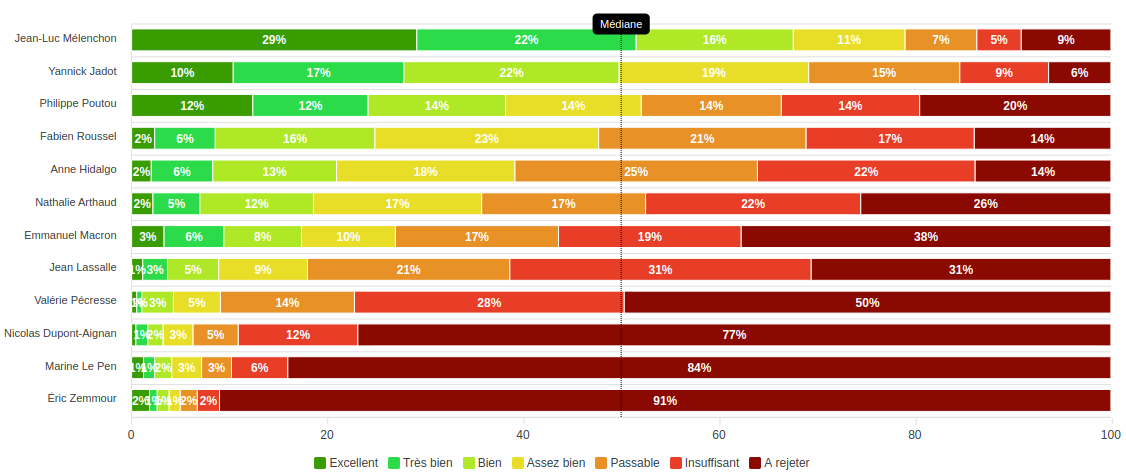
\includegraphics[scale=0.3]{data/profileUAV}
		\label{fig:distributionUAVFrench}
	\end{figure}
	
	\begin{figure}
		\centering
		\caption{Probabilité moyenne de ne pas trouver le gagnant en utilisant une distribution des préférences de cas réel, étant donné $m=12$ pour $n\in \{10,25,50,100,250,500\}$ et $k\in \intvl{1,5}$.}
		\label{fig:MJelicitationUAVFrench}
		\begin{tikzpicture}[scale=0.6]
			\pgfplotsset{
				every axis legend/.append style={
					at={(0.5,1.1)},
					anchor=south
				},
			}
			\begin{axis}[
				%	y=8,
				xlabel=$k$,
				ylabel=Avg. Prob. of Miss.,
				table/col sep=comma,
				legend columns=3,
				%	ytick={0,2,4,6,8,10},
				%	xtick distance=10,
				%	ytick distance=2,
				%	xtick pos=left,
				ymajorgrids=true,
				ytick style={draw=none},
				ymin=0,
				ymax=0.8,
				xmin=1,
				xmax=5,
				yticklabels={0,2,4,6,8,10},
				legend style={font=\scriptsize}
				]
				
				\addlegendimage{mark=halfsquare right*,brown,mark size=2}
				\addlegendimage{mark=diamond*,red,mark size=2}
				\addlegendimage{mark=pentagon*,cyan,mark size=2}
				\addlegendimage{mark=halfcircle*,violet,mark size=2}
				\addlegendimage{mark=*,pink,mark size=2}
				\addlegendimage{mark=triangle*,green,mark size=2}
				\addlegendimage{mark=halfsquare left*,blue,mark size=2}
				\addlegendimage{mark=square*,teal,mark size=2}
				\addlegendimage{mark=halfsquare*,magenta,mark size=2}
				
				
				\addplot[thick, mark=halfsquare right*, mark size = {2}, mark indices = {3}, brown] table [x=k, y=p10]{data/electiontableFig.dat};
				\addlegendentry{n=10}
				\addplot[thick, mark=diamond*, mark size = {2}, mark indices = {3}, red] table [x=k, y=p25]{data/electiontableFig.dat};
				\addlegendentry{n=25}
				\addplot[thick, mark=pentagon*, mark size = {2}, mark indices = {2}, cyan] table [x=k, y=p50]{data/electiontableFig.dat};
				\addlegendentry{n=50}
				\addplot[thick, mark=halfcircle*, mark size = {2}, mark indices = {2}, violet] table [x=k, y=p100]{data/electiontableFig.dat};
				\addlegendentry{n=100}
				\addplot[thick, mark=*, mark size = {2}, mark indices = {1}, pink] table [x=k, y=p250]{data/electiontableFig.dat};
				\addlegendentry{n=250}
				\addplot[thick, mark=triangle*, mark size = {2}, mark indices = {1}, green] table [x=k, y=p500]{data/electiontableFig.dat};
				\addlegendentry{n=500}
				%				\addplot[thick, mark=halfsquare left*, mark size = {2}, mark indices = {1}, blue] table [x=k, y=p1000]{data/electiontableFig.dat};
				%				\addlegendentry{n=1000}
				%				\addplot[thick, mark=square*, mark size = {2}, mark indices = {1}, teal] table [x=k, y=p1500]{data/electiontableFig.dat};
				%				\addlegendentry{n=1500}
				
			\end{axis}
		\end{tikzpicture}
	\end{figure}

\newpage
\section{Compromising as an equal loss principle}
	Le mot compromis vient du latin \textit{compromissus}, participe passé de \textit{compromittere} : com \textit{ensemble} et promittere \textit{promettre}.
	L'idée de compromis se retrouve en effet dans des textes datant de l'époque romaine, où deux parties en conflit qui souhaitaient soumettre leur différend à l'arbitrage désignaient un tiers (un arbitre) et promettaient mutuellement de se conformer au jugement incontestable de ce dernier. Si l'une des parties avait rompu cette promesse, elle aurait dû payer une pénalité.
	Dans un fragment d'une lettre écrite par Proculus, qui est rapporté par \citet [p.529]{Zimmermann1996}, il est clair que les deux parties au conflit ont accepté de donner à l'arbitre des pouvoirs illimités dans sa décision. Aucun recours n'était possible contre la sentence finale, qui était contraignante, aussi injuste et inégale soit-elle. Cette idée du compromis comme simple processus d'arbitrage semble très différente de la notion que nous en avons aujourd'hui. Considérons les définitions des deux verbes dans un dictionnaire moderne : arbitrer "régler un différend entre deux personnes ou groupes après avoir entendu les arguments et les opinions de chacun" ; compromettre "parvenir à un accord par concession mutuelle".
	La concession mutuelle est l'élément qui nous fait immédiatement penser à un compromis et c'est précisément le facteur manquant dans la description du compromis romain et de l'arbitrage moderne. En citant \citet{Braybrooke1982} \say{C'est tout simplement une mauvaise plaisanterie que de dire qu'une personne est partie à un compromis alors qu'elle n'en a rien retiré.}.
	
	Dans \Cref{ch:compromise}, nous présentons deux versions différentes de compromis, en particulier une qui privilégie l'égalité aux dépens de l'efficacité de Pareto. De plus, nous considérerons le concept de "equal-loss" (perte égale) \citep{Chun1988, Chun1991} comme la base du compromis dans toutes les situations où l'égalitarisme, au sens de concéder également, est une prérogative importante.
	Il s'agit d'une nouveauté dans la littérature des règles de choix social, qui jusqu'à présent n'ont fait qu'imposer la volonté de compromis sans réellement garantir que toutes les parties concèdent quelque chose.
	Le philosophe \citet{Day1989} tente d'expliquer ce phénomène en pensant qu'il découle de la négation de l'adjectif "intransigeant" : 
	\textit{\say{Une personne intransigeante est une personne qui n'est pas disposée à faire des concessions, donc (on en déduit à tort) une personne compromettante est une personne souple et disposée à faire des concessions\textemdash indépendamment du fait qu'elle reçoive une concession en retour. Quoi qu'il en soit, il faut insister, car il est généralement admis que le compromis implique nécessairement des concessions mutuelles.}}
	Cela pourrait expliquer pourquoi toutes les règles de vote qui tentent de faire un compromis se contentent en fait de la volonté des agents de faire un compromis. 
	
	\cite{Merlin2019} discutent des plus célèbres de ces procédures en proposant de les rassembler dans la même classe de \textit{règles de compromis}.
	Dans \Cref{sec:BK}, nous avons déjà défini le \acl{MC}, introduit par \citet{Sertel1986} et analysé plus en détail par \citet{Sertel1999}. Basée sur une révision de la règle de Condorcet-Bucklin, cette procédure part du choix idéal de chacun pour trouver une alternative soutenue par la majorité des votants. Si une telle alternative n'existe pas, elle se rabat sur le deuxième, le troisième et plus généralement le $k$-\emph{e} meilleur choix des votants, jusqu'à ce qu'au moins une des alternatives considérées figure parmi les $k$ premiers meilleurs pour une majorité.
	Si au lieu de considérer un accord pour la majorité des votants, nous souhaitons sélectionner comme gagnants les alternatives soutenues par l'unanimité des votants, alors la procédure correspond à la règle \acl{FB}. 
	Plus généralement, si nous considérons le soutien d'un certain quota $q$ d'électeurs, nous nous référons à la règle de "q-approval fallback bargaining" \citep{Brams2001}.
	
	Toutes ces \acp{SCR} imposent aux électeurs une volonté de compromis, mais nous soutenons qu'elles ne garantissent pas efficacement un résultat où les agents ont effectivement fait des compromis. Cet exemple motive notre point de vue:
	
	\begin{example}
		Considérons le profil de préférence suivant avec $n=100$:
		\begin{center}
			$
			\begin{array}{cc}
				\mathbf{49} & \mathbf{51} \\
				c	&	a	\\
				b	&	b	\\
				a	&	c	\\
			\end{array} \quad.
			$
		\end{center}
		Lorsque $q\in \intvl{1,\frac{n}{2}+1} $, tous les compromis BK choisissent $a$ et $c$ tandis que les compromis BK révisés choisissent $a$. Ces résultats n'apparaissent pas comme un compromis car près de la moitié des votants obtiennent leur meilleur choix tandis que l'autre moitié doit se contenter de leur pire choix. Observez que $b$ reçoit un soutien unanime lorsque chaque électeur recule d'un pas par rapport à son point idéal.
	
		When $q\in \intvl{1,\frac{n}{2}+1} $, all BK compromises pick $a$ and $c$ while the revised BK compromises select $a$. These outcomes do not appear as a compromise as almost half of the voters obtain their best choice while the remaining half have to be contented with their worst one. Observe that $b$ receives unanimous support when each voter falls back one step from her ideal point.
	\end{example}
	
	Nous définissons qu'une règle est \textit{Egalitarian Compromise} (EC) (resp., \textit{Egalitarian Compromise Compatible} (ECC)), si \emph{tous} (resp., \emph{quelques}) les gagnants sont parmi les alternatives avec les pertes les plus également distribuées. Évidemment, EC est une sous-classe de ECC.
	
	De plus, nous définissons qu'une règle est \textit{Paretian Compromise} (PC) (resp., \textit{Paretian Compromise Compatible} (PCC)), si \emph{tous} (resp., \emph{quelques}) les gagnants sont parmi les alternatives Pareto optimales avec les pertes les plus également distribuées. Évidemment, PC est une sous-classe de PCC.

	\paragraph{Conclusions.}
	Nous prouvons que : aucune procédure de Condorcet n'est ECC ou PCC (\Cref{th:condorcet}), aucune règle de score n'est ECC (\Cref{th:srECC}) ou PCC à l'exception de la règle d'antipluralité (\Cref{th:AntSatsPCC,th:srPCC}), les compromis \acs{BK} ne sont ni ECC ni PCC (\Cref{th:BKthreshold,th:FBfailsECC}) à l'exception de fallback bargaining qui est PC (\Cref{th:FBsatsPC}).
	
	Nos résultats d'impossibilité sont énoncés pour l'ensemble des mesures d'écart $\Sigma$, mais ils prévalent pour tout sous-ensemble de $\Sigma$. Comme $\Sigma$ est le plus grand ensemble de mesures d'écart sensibles, ils sont valables pour tout concept spécifique d'équité que l'on pourrait choisir. D'autre part, nos résultats de possibilité sur le fallback bargaining et l'antipluralité ne se propagent pas aux sous-ensembles de $\Sigma$. En fait, dès qu'une restriction raisonnablement légère sur $\Sigma$ est imposée, les deux règles ne sont plus PCC (\Cref{th:3votRestriction}). Avec deux individus et une restriction similaire sur $\Sigma$, tous les SCR à deux personnes bien connus de la littérature, à savoir le fallback bargaining, les règles de fallback bargaining, Pareto and veto rules, short listing et veto rank, ne parviennent pas à trouver des compromis ex-post (\Cref{th:2votPCC}).
	
	L'exclusion du principe d'égalité des pertes par la quasi-totalité de la littérature conduit à se demander si le principe ne présente pas d'intérêt dans un contexte de choix social discret. Cela semble être le cas pour les situations de vote où le nombre d'électeurs dépasse le nombre de candidats et où, en général, chaque candidat est classé dernier par au moins un électeur. Dans ces cas, la principale préoccupation concerne le soutien des alternatives plutôt que l'égalité. D'autre part, les problèmes de choix collectifs à deux personnes sont généralement interprétés comme des situations d'arbitrage ou de négociation où le consentement mutuel est un élément essentiel pour parvenir à une solution. Ainsi, le principe de perte égale semble être valide pour les problèmes de choix collectifs à deux personnes et notre analyse soulève la question de la conception de nouvelles règles d'arbitrage discrètes compatibles avec le principe de perte égale.

\section{Conclusions et Perspectives}
	Tout au long de ce manuscrit, nous avons abordé plusieurs problèmes liés au domaine du choix social. En particulier, nous nous sommes concentrés sur deux scénarios. 
	En considérant un modèle classique dans lequel les préférences d'un ensemble de votant sont connues, nous avons défini deux classes de règles de vote capables de refléter une notion de compromis dans laquelle l'égalitarisme, au sens de concéder également, est une préoccupation majeure.
	En outre, nous avons pris de la distance par rapport à cette perspective standard dans laquelle les préférences sont supposées être connues dès le départ et nous avons étudié le problème de l'élicitation des préférences dans différents contextes.
	
	Il existe de nombreuses directions intéressantes pour les travaux futurs pour chacun des problèmes considérés.
	En ce qui concerne l'élicitation simultanée des règles de vote et des préférences des agents, on pourrait développer davantage de stratégies avec différentes heuristiques pour les comparer à celles que nous avons proposées. Par exemple, des stratégies moins coûteuses en calcul permettraient de tester des ensembles de données plus importants, avec plus de votants et plus d'alternatives. 
	Il serait également intéressant d'étendre l'élicitation des règles de vote autres que les règles de position. 
	En outre, nous pensons que la transformation des questions en profils d'exemple est un concept très intéressant qui n'est pas beaucoup exploré dans la littérature et qui pourrait être appliqué dans différents contextes. 
	
	Le chapitre consacré à l'analyse de la procédure d'élicitation à l'aide de MJ n'est pas encore tout à fait terminé, de sorte qu'il existe de nombreuses idées d'extensions possibles. On pourrait, par exemple, étudier la possibilité de manipuler le processus d'élicitation lui-même. En particulier, comment la partie chargée d'interroger les électeurs peut manipuler le résultat en dirigeant les questions vers des électeurs spécifiques. 
	Une autre piste peut concerner l'explicabilité de ce processus. Les électeurs peuvent avoir du mal à croire que le fait de juger une seule personne donne une bonne approximation du résultat qui serait obtenu en demandant le profil complet.
	
	Enfin, lorsque l'on considère le concept de compromis, différentes notions de compromis peuvent être conçues. Une approche pourrait consister à choisir des alternatives qui ne sont ni les meilleures ni les pires d'un électeur. Tout dépend de l'idée de justice que l'on veut représenter et des priorités du scénario considéré.
	En outre, le compromis entre équité et efficacité peut être exploré dans d'autres contextes, plus riches. 
	Pour conclure, nous aimons penser que chacune de nos contributions n'est que le début d'une longue série de développements futurs.
